% This paper follows the LLNCS macro package for Springer Computer Science
% proceedings; based on samplepaper.tex, Version 2.21 of 2022/01/12.
%
% English edition of reports/lncs_phuong_phap.tex. The Vietnamese file is kept
% as-is; the two are meant to stay in step, so a change to one belongs in the
% other as well.
%
\documentclass[runningheads]{llncs}
%
% ---------------------------------------------------------------------
% FONT ENCODING
% The body of this paper is English, for which the sample's [T1] would be
% correct. We keep [T5] for one reason only: the author names carry Vietnamese
% diacritics that T1 cannot render. T5 covers the full ASCII range, so English
% text sets exactly as it would under T1.
% ---------------------------------------------------------------------
\usepackage[utf8]{inputenc}
\usepackage[T5]{fontenc}
%
\usepackage{graphicx}
\usepackage{amsmath}
\usepackage{amssymb}
% The pipeline figure is drawn in TikZ, i.e. vector graphics, as the sample
% recommends for diagrams and schematics.
\usepackage{tikz}
\usetikzlibrary{arrows.meta, positioning}
%
\begin{document}
%
% No \renewcommand block here: llncs already labels everything in English.
%
\title{Two-Stage Fusion for Routing and Classification in
Parameter-Efficient Continual Learning}
%
\titlerunning{Two-Stage Fusion for PET-Based Continual Learning}
%
% ORCID iDs not yet available; \orcidID{} omitted for now. Fill in before
% the final submission.
\author{Nguyễn Thiên Trường \and Tống Quang Thái}
%
\authorrunning{N. T. Trường and T. Q. Thái}
%
% Add e-mail addresses before submitting.
\institute{University of Engineering and Technology,\\
Vietnam National University, Hanoi, Vietnam}
%
\maketitle
%
\begin{abstract}
Continual learning methods built on parameter-efficient tuning maintain a
lightweight parameter pool, one set per task, and at inference must decide which
set to attach to the backbone before classifying. That decision is made from a
single source of evidence, so everything downstream is capped by the quality of
one module. We show that a second source of evidence is already present inside
the trained model and can be exploited without training a single additional
parameter: a second-order classification head built on a frozen random
projection of the existing LoRA features. This source is fused at two points,
both at inference time. The first stage blends it with the original routing
signal after standardising the two sources onto a common scale. The second stage
uses it as a secondary classifier, weighted per sample in inverse proportion to
how decided the primary classifier already is, so that the blend opens only on
contested samples. Across three continual-learning benchmarks and four seeds,
routing accuracy rises by $+1.10$ to $+2.26$ points and classification accuracy
by $+0.69$ to $+1.50$ points; on both axes the gain is several times the
seed-to-seed standard deviation. The two retention metrics show no change
distinguishable from zero. The added cost is exactly one forward pass per
sample.

\keywords{Continual learning \and Parameter-efficient tuning \and Parameter
routing \and Random projection \and Signal fusion.}
\end{abstract}
%
%
%
\section{Introduction}

A continual learner built on parameter-efficient tuning keeps one lightweight
parameter set per task and, at inference, must decide which set to attach to the
frozen backbone before it can classify. That decision is made once, from a
single module, and everything downstream inherits it: a wrong choice attaches
the wrong adapter, and the classifier that follows is asked to work from
features it was not adapted for. Successive methods in this line have improved
the decision --- richer pools, attention-weighted combinations, explicit
re-matching stages --- but none change the fact that one signal stands in front
of the rest of the pipeline.

We observe that a second, independent source of evidence is already present
inside such a trained model and is simply discarded. The LoRA features that the
pipeline computes anyway can be pushed through a fixed random projection and
read by a closed-form ridge classifier built from second-order statistics. This
head trains no parameters, stores no images, and costs one forward pass that the
pipeline already performs. More importantly it fails on \emph{different samples}
than the routing module does, which is the property that makes combining them
worthwhile rather than redundant.

The paper puts that second source to work at the two points where the original
pipeline commits to a decision. At the routing level it is blended with the
existing task signal after both are standardised onto a common scale. At the
classification level it is used as what it already is --- a complete classifier
--- weighted per sample so that the blend opens only where the primary
classifier is undecided.

\subsubsection{Contributions.}
\begin{itemize}
\item We identify two weaknesses in the re-matching pipeline of
      HRM-PET~\cite{ref_hrmpet}: its routing signal comes from one module, and a
      better route does not automatically become a better prediction because the
      shared head frequently predicts the correct class in spite of a wrong
      route (Sect.~\ref{sec:method}).
\item We show that a training-free second-order head over a frozen random
      projection of the existing features supplies a second source of evidence
      whose errors are decorrelated from the first, and we fuse the two at both
      the routing and the classification level, entirely at inference time.
\item We evaluate on three datasets over four seeds and report by axis: routing
      improves by $+1.10$ to $+2.26$ points and classification by $+0.69$ to
      $+1.50$, each several times the seed-to-seed standard deviation, while the
      two retention metrics show no change we can resolve and we claim none
      (Sect.~\ref{sec:results}).
\item We reconstruct the full grid the original work covers --- four datasets by
      five pre-training configurations, identified from traces in its released
      code --- and add MAE as a twenty-first cell. All $21$ improve on both
      accuracy axes, with the largest gain on the weakest backbone
      (Sect.~\ref{sec:grid}).
\end{itemize}

\subsection{Problem Statement}

Class-incremental learning (CIL) learns a sequence of $T$ tasks without
forgetting earlier ones. The $t$-th task consists of $n_t$ samples
$\mathcal{D}_t=\{(x^t_i,y^t_i)\}_{i=1}^{n_t}$ drawn from a class set
$\mathcal{C}_t$, where $x^t_i \in \mathcal{X}$ is an input image and
$y^t_i \in \mathcal{Y}$ its label.

Three constraints define the setting. At step $t$ only $\mathcal{D}_t$ is
available for training. The class sets are disjoint,
$\mathcal{C}_t \cap \mathcal{C}_{t'} = \emptyset$ for all $t \neq t'$, and at
inference the \emph{task identity is unknown}: the model must discriminate among
all classes seen so far through a single shared classification head. Finally,
this work operates in the exemplar-free setting: images from past tasks are
never retained.

In methods based on parameter-efficient tuning
(PET)~\cite{ref_l2p,ref_dualprompt,ref_hide}, a pre-trained backbone
$h_{\mathrm{ptm}}$ with parameters $\theta_{\mathrm{ptm}}$ is frozen and a
lightweight parameter pool $\mathcal{P}=\{p_1,\dots,p_T\}$ is maintained, each
set trained on one task; here every $p_t$ is a LoRA adapter~\cite{ref_lora}. The
shared classification head is denoted $g_{\theta_g}$. Because the task identity
is unknown at inference, the system is forced to \emph{choose} which parameter
set to attach to the backbone before classifying, and everything downstream
depends on that choice. Table~\ref{tab:notation} summarises the notation used
throughout.

\begin{table}
\caption{Notation used in this paper.}\label{tab:notation}
\begin{tabular}{ll}
\hline
Symbol & Meaning\\
\hline
$\mathcal{D}_t$, $\mathcal{C}_t$ & data and class set of task $t$\\
$h_{\mathrm{ptm}}$, $\theta_{\mathrm{ptm}}$ & pre-trained backbone, frozen\\
$\mathcal{P}=\{p_1,\dots,p_T\}$ & LoRA parameter pool, one set per task\\
$g_{\theta_g}$, $g_\omega$ & shared classification head; auxiliary classifier of TII\\
$q(x)$ & query feature from the bare backbone\\
$\hat{d}(x)$, $\tilde{d}(x)$ & class distribution of TII; of the routed classifier\\
$\mathcal{T}(\cdot)$ & map from class to task identity\\
$\hat{t}_f$, $\hat{t}_s$ & task identity at first matching and after re-matching\\
$\ell \in \mathbb{R}^{|\mathcal{Y}|}$ & class scores of the routed classifier\\
$s \in \mathbb{R}^{|\mathcal{Y}|}$ & class scores of the random-projection head\\
$z(\cdot)$ & per-sample standardisation to zero mean and unit variance\\
\hline
\end{tabular}
\end{table}

\subsection{The HRM-PET Baseline Pipeline}

We take HRM-PET~\cite{ref_hrmpet} as our baseline. Its inference pipeline
consists of four modules in sequence, presented in the order the data passes
through them.

\subsubsection{Task-identity inference (TII).}
The input image is passed through the \emph{bare} backbone, with no adapter
attached, to obtain a query feature. That feature enters an auxiliary classifier
$g_\omega$ trained with cross-entropy, producing a distribution over classes:
\begin{equation}
q(x) = h(x;\theta_{\mathrm{ptm}}),
\qquad
\hat{d}(x) = g\!\left(q(x); \theta_\omega\right).
\label{eq:tii}
\end{equation}
The initial task identity is the task containing the highest-probability class,
with $\mathcal{T}$ the class-to-task map.

\subsubsection{Direct re-matching (DRM).}
Thanks to the knowledge shared across the parameter pool, for some samples the
class predicted by the classifier \emph{already} belongs to the correct task
even when the initial match was wrong. Such samples are identifiable because the
predicted class does not belong to the matched task:
\begin{align}
\hat{t}_f &= \mathcal{T}\!\left(\arg\max_i\, g(q(x);\theta_\omega)\right),
\label{eq:tf}\\
\hat{t}_s &= \mathcal{T}\!\left(\arg\max_i\,
   g\!\left(h(x; p_{\hat{t}_f}, \theta_{\mathrm{ptm}}); \theta_g\right)\right),
\label{eq:ts}
\end{align}
and HRM-PET substitutes only when the two disagree:
\begin{equation}
\hat{y} =
\begin{cases}
\arg\max_i\, g\!\left(h(x; p_{\hat{t}_s}, \theta_{\mathrm{ptm}}); \theta_g\right),
  & \text{if } \hat{t}_f \neq \hat{t}_s,\\[2pt]
\arg\max_i\, g\!\left(h(x; p_{\hat{t}_f}, \theta_{\mathrm{ptm}}); \theta_g\right),
  & \text{otherwise.}
\end{cases}
\label{eq:drm}
\end{equation}
If $\hat{t}_s$ is correct, routing accuracy improves; if it is wrong, the worst
outcome is a wrong prediction that $\hat{t}_f$ was already going to produce. The
design therefore cannot degrade performance.

\subsubsection{Confidence-based re-matching (CRM).}
When $\hat{t}_f = \hat{t}_s$, DRM has nothing to substitute. For those samples
HRM-PET relies on the observation that each parameter set was trained only
alongside the classes of its own task, so for a mismatched sample the predictive
distribution tends to be less decided. The confidence $E(\cdot)$ is computed as a
generalised posterior entropy, requiring no extra training, and a detector
compares it against a threshold $\tau$:
\begin{equation}
De(x) =
\begin{cases}
0, & \text{if } E(\tilde{d}(x)) \leq \tau \quad (\text{suspected mismatch}),\\
1, & \text{otherwise.}
\end{cases}
\label{eq:detect}
\end{equation}
Since no sharp boundary can be drawn by $\tau$ alone, HRM-PET does not replace
$\hat{t}_f$ outright but compares confidences across a candidate set $\Gamma$ of
the $N$ highest-probability classes in $\hat{d}(x)$:
\begin{equation}
\hat{t}_s = \arg\max_{i \,\in\, \Gamma}\;
   E\!\left(g\!\left(h(x; p_{\mathcal{T}(i)}, \theta_{\mathrm{ptm}});
   \theta_g\right)\right),
\qquad N = 2 .
\label{eq:crm}
\end{equation}
Each candidate costs one additional forward pass, so $N$ is kept small.

\subsubsection{Shared classification head.}
The selected parameter set is attached to the backbone, and the shared head
produces a score vector over all classes seen so far:
\begin{equation}
\ell = g\!\left(h(x; p_{\hat{t}}, \theta_{\mathrm{ptm}}); \theta_g\right)
   \in \mathbb{R}^{|\mathcal{Y}|},
\qquad
\hat{y} = \arg\max_c\, \ell_c ,
\label{eq:logits}
\end{equation}
where $\hat{t}$ is the identity after DRM and CRM. Classes not yet seen are
masked with $-\infty$.

\subsubsection{Two weaknesses of this structure.}
First, the whole four-module chain depends on \emph{one} routing signal,
produced at (\ref{eq:tii}); DRM and CRM only refine it and add no further
source. Second, $\ell$ in (\ref{eq:logits}) comes from the \emph{shared} head,
so it frequently predicts the correct class in spite of a wrong routing
decision --- improved routing therefore does not automatically translate into
improved classification. These two points lead directly to the two components
proposed in Sect.~\ref{sec:method}.

\section{Related Work}
\label{sec:related}

\subsubsection{Parameter pools and the selection they require.}
L2P~\cite{ref_l2p} and DualPrompt~\cite{ref_dualprompt} established the shape
that most parameter-efficient continual learners still follow: freeze the
backbone, keep a pool of lightweight parameter sets, and pick from the pool at
inference using a query computed from the bare backbone. CODA-Prompt~\cite{ref_coda}
replaces the discrete pick with an attention-weighted combination, and
HiDe-Prompt~\cite{ref_hide} makes the structure explicit by decomposing the
problem into within-task prediction, task-identity inference and task-adaptive
prediction, then optimising the three separately; its central observation is
that task-identity inference, not within-task classification, is what limits the
whole pipeline. HRM-PET~\cite{ref_hrmpet}, our baseline, belongs to this line: it
substitutes LoRA adapters~\cite{ref_lora} for prompts and adds re-matching stages
that revisit the initial task decision. Recent work continues to enlarge the
pool rather than change its structure --- MoTE~\cite{ref_mote} keeps one
task-specific expert per task and filters them at inference, and dynamic
LoRA-expert selection with prototype matching~\cite{ref_dlepem} does the same
with prototypes as the matching signal. All of these share the property this
paper targets: a single selection decision stands in front of the classifier,
and everything downstream inherits its errors.

\subsubsection{Classifiers that are never trained.}
A separate line abandons routing altogether and reads the frozen features
directly. Nearest-class-mean prototypes are the simplest instance; ADaM and its
successors~\cite{ref_adam} adapt the backbone on the first task only and then
freeze it; RanPAC~\cite{ref_ranpac} projects the frozen features through a fixed
random matrix, accumulates second-order statistics, and solves a ridge system in
closed form. These methods are strong: on Split-ImageNet-R with a ViT-B/16
backbone, RanPAC reports $77.9\%$ where a linear probe trained jointly on all
$200$ classes --- a model that by construction cannot forget --- reaches
$72.0\%$~\cite{ref_ranpac}. The comparison is worth stating plainly, because it
sets the terms of our own: a training-free head over frozen features is not a
weak fallback, and the gap between such a head and a routed pipeline is not
explained by forgetting. What these methods give up is the structure that
routing provides. We take the head of~\cite{ref_ranpac} and use it inside a
routing pipeline as a second source of evidence rather than as a replacement for
the first.

\subsubsection{Correcting the classifier after the fact.}
Class-incremental classifiers are biased towards recently seen classes, and the
survey of Masana et al.~\cite{ref_survey} locates that bias concretely: both the
bias terms and the norms of the classifier weights grow with task recency.
Corrections follow the diagnosis. iCaRL~\cite{ref_icarl} sidesteps the learned
weights by classifying to the nearest exemplar mean; BiC~\cite{ref_bic} learns a
per-task affine map on top of the logits using a held-out validation split;
Weight Aligning~\cite{ref_wa} rescales the new-class weight vectors so their mean
norm matches the old ones; LUCIR~\cite{ref_lucir} removes the norm asymmetry
structurally by normalising both features and weights before the softmax. Our
setting rules most of this out rather than improving on it: we hold no exemplars
and no validation split, and we never touch training --- the adapters, the
auxiliary classifier and the shared head all arrive frozen. The fusion described
in Sect.~\ref{sec:method} therefore has to act on scores alone, at inference,
from quantities already present in the forward pass.

\section{Method}
\label{sec:method}

We add a second source of evidence and two places at which to fuse it in, one
for each weakness above. Both sit at inference time: no parameter is trained and
no model is retrained. Figure~\ref{fig:pipeline} shows where they go.

% [!ht] rather than the sample's bare \begin{figure}: the reference to this
% figure is the last sentence of the section opening, so the figure has to sit
% directly under it. The default tbp lets it drift pages away from its mention.
\begin{figure}[!ht]
\centering
\resizebox{\textwidth}{!}{%
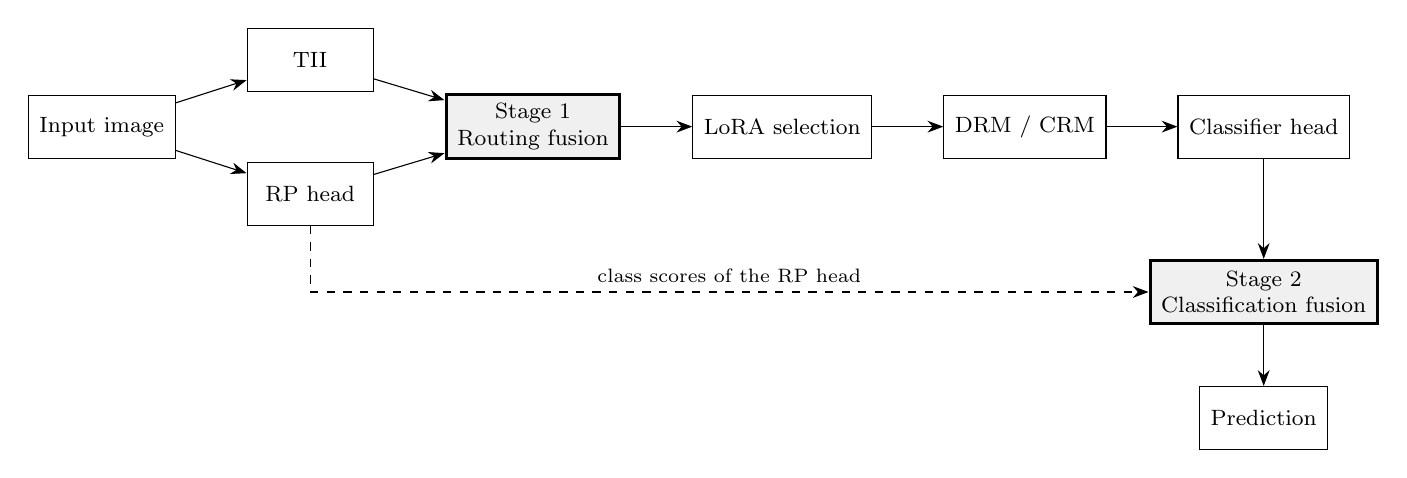
\begin{tikzpicture}[
  font=\footnotesize,
  >={Stealth[length=2mm]},
  box/.style={draw, minimum height=8mm, minimum width=1.6cm, inner xsep=4pt, align=center},
  hl/.style={box, very thick, fill=black!6}
]
% Each box is chained off the previous one's east edge, so what is specified is
% the GAP and the width is free to be whatever the label needs. Fixed centre
% coordinates cannot work here: box width depends on label length, so longer
% words silently eat the gap. With the old centres the LoRA-to-DRM gap fell to
% 1.49pt against a 2mm (5.69pt) arrow tip, i.e. the arrowhead was drawn inside
% the neighbouring box. 9mm keeps every gap at 25.61pt in both languages.
\node[box] (in) at (0, 0) {Input image};
\coordinate (up) at (0, 0.85);
\coordinate (dn) at (0,-0.85);
\coordinate (r1) at ([xshift=9mm]in.east);
\node[box, anchor=west] (tii) at (r1 |- up) {TII};
\node[box, anchor=west] (rp)  at (r1 |- dn) {RP head};
% anchored on rp, not tii: rp carries the longer label of the two, so it is the
% binding constraint if either label is ever edited.
\coordinate (r2) at ([xshift=9mm]rp.east);
\node[hl,  anchor=west] (f1) at (r2 |- in) {Stage 1\\Routing fusion};
\node[box, anchor=west] (lo) at ([xshift=9mm]f1.east) {LoRA selection};
\node[box, anchor=west] (dr) at ([xshift=9mm]lo.east) {DRM / CRM};
\node[box, anchor=west] (cl) at ([xshift=9mm]dr.east) {Classifier head};
\node[hl]  (f2) at ([yshift=-2.1cm]cl.center) {Stage 2\\Classification fusion};
\node[box] (out) at ([yshift=-3.7cm]cl.center) {Prediction};
\draw[->] (in) -- (tii);
\draw[->] (in) -- (rp);
\draw[->] (tii) -- (f1);
\draw[->] (rp) -- (f1);
\draw[->] (f1) -- (lo);
\draw[->] (lo) -- (dr);
\draw[->] (dr) -- (cl);
\draw[->] (cl) -- (f2);
\draw[->] (f2) -- (out);
\draw[->, dashed] (rp.south) |- node[pos=0.75, above, font=\scriptsize]
      {class scores of the RP head} (f2.west);
\end{tikzpicture}}
\caption{The inference pipeline. The bold-outlined blocks are the two added
components. The random-projection head is computed exactly once and feeds both
stages: task scores for the first, class scores for the second (dashed line).}
\label{fig:pipeline}
\end{figure}

\subsection{The Second Source of Evidence}

The second source must satisfy two constraints: it must add no trainable
parameters, since parameters updated by gradients across a task sequence can be
overwritten by later tasks; and it must preserve the exemplar-free protocol. A
second-order classification head in the style of RanPAC~\cite{ref_ranpac}
satisfies both.

The input feature $f \in \mathbb{R}^{d}$ with $d = 768$ is taken from the final
feature layer of ViT-B/16 after attaching \emph{one} fixed LoRA parameter set,
which serves as first-session adaptation. The index of that parameter set must be
fixed across all tasks; otherwise the accumulated terms below would mix
incompatible feature spaces.

\subsubsection{Projection and second-order statistics.}
The feature is projected into a high-dimensional space of size $M = 10^4$ and
passed through a nonlinearity, and the projected features are accumulated into
two matrices:
\begin{align}
h &= \mathrm{ReLU}(f W) \in \mathbb{R}^{M},
\qquad W \in \mathbb{R}^{d \times M} \text{ frozen, drawn from a fixed seed},
\label{eq:proj}\\
G &= \sum_n h_n h_n^{\top} \in \mathbb{R}^{M \times M},
\qquad
C = \sum_n h_n\, \mathbf{e}_{y_n}^{\top}
   \in \mathbb{R}^{M \times |\mathcal{Y}|},
\label{eq:gram}
\end{align}
where $\mathbf{e}_{y}$ is the basis vector of class $y$. The sums run over every
sample seen since the start of the sequence.

Going up in dimension is deliberate: in the original $768$-dimensional space the
classes overlap to the point that no hyperplane separates them, whereas after
the expansion a linear classifier becomes expressive enough. The nonlinearity is
mandatory rather than optional --- without it $fW$ is merely a linear transform
of $f$, of rank at most $d$, and projecting into $M \gg d$ dimensions adds no
separating power whatsoever.

\subsubsection{Classification by ridge regression.}
The output weights are the closed-form solution of a regularised least-squares
problem:
\begin{equation}
W_{\mathrm{out}} = (G + \lambda I)^{-1} C \in \mathbb{R}^{M \times |\mathcal{Y}|},
\qquad
s = h^{\top} W_{\mathrm{out}} \in \mathbb{R}^{|\mathcal{Y}|} .
\label{eq:ridge}
\end{equation}
There is no separate dimensionality-reduction step: $W_{\mathrm{out}}$ performs
it, collapsing $M$ dimensions down to $|\mathcal{Y}|$ in a single matrix
product. The trajectory of dimensions is
\begin{center}
$\underbrace{768}_{f}
\;\xrightarrow{\;\text{projection} + \text{nonlinearity}\;}\;
\underbrace{10^4}_{h}
\;\xrightarrow{\;W_{\mathrm{out}}\;}\;
\underbrace{|\mathcal{Y}|}_{s}$
\end{center}
We go up \emph{in order to make} the linear step down work. The Gram inverse is
the component that makes it work: the post-nonlinearity dimensions are strongly
correlated, and $(G + \lambda I)^{-1}$ decorrelates them.

\subsubsection{Two inherited properties.}
Both $G$ and $C$ in (\ref{eq:gram}) are \emph{sums} over samples, and addition
commutes. Consequently $W_{\mathrm{out}}$ does not depend on the order in which
the tasks were learned: this head does not forget, in a structural sense, rather
than by virtue of some anti-forgetting mechanism added on top. At the same time
the sizes of the two matrices do not depend on how many samples have been seen,
and no per-sample feature is ever retained, so the exemplar-free protocol is
preserved by the structure of the computation itself.

\subsection{Two-Stage Fusion}

Both stages blend two vectors that live on different scales: the ridge scores $s$
span roughly one unit while the logits $\ell$ span roughly thirty-five, so a
direct blend would let $\ell$ dominate at every weight. Each source is therefore
standardised per sample before blending:
\begin{equation}
z(v) = \frac{v - \mathrm{mean}(v)}{\mathrm{std}(v)} ,
\label{eq:znorm}
\end{equation}
with the mean and standard deviation computed separately for each sample, over
the classes seen so far only.

\subsubsection{First stage: fusion at the routing level.}
Both sources emit scores over \emph{classes}, whereas routing needs scores over
\emph{tasks}. We convert by taking the maximum over each task's class set, since
a task deserves to be selected when \emph{some} class of its own scores highly,
not when its classes score highly on average:
\begin{equation}
\ell^{\mathrm{task}}_t = \max_{c \in \mathcal{C}_t} \ell_c ,
\qquad
s^{\mathrm{task}}_t = \max_{c \in \mathcal{C}_t} s_c ,
\qquad t = 1,\dots,\hat{T},
\label{eq:taskscore}
\end{equation}
with $\hat{T}$ the number of tasks seen so far. The two vectors are blended
after standardisation:
\begin{equation}
\mathrm{fused} = w\, z(\ell^{\mathrm{task}}) + (1-w)\, z(s^{\mathrm{task}}),
\qquad
\hat{t}_f = \arg\max_t\, \mathrm{fused}_t ,
\qquad w = 0.7 .
\label{eq:route}
\end{equation}
The identity $\hat{t}_f$ replaces the output of (\ref{eq:tii}) and is handed to
DRM and CRM as a better starting point. We replace \emph{exactly one} module, the
first matching step; every downstream mechanism is left untouched. At $w = 1.0$,
(\ref{eq:route}) returns exactly the ordering of $\ell^{\mathrm{task}}$, so the
method reduces to the baseline.

\subsubsection{Second stage: gated fusion at the classification level.}
Because $\ell$ comes from the shared head, it frequently predicts the correct
class in spite of a wrong routing decision. We therefore use the
random-projection head itself as a secondary classifier, this time taking its
class scores $s$.

A fixed weight is the wrong instrument. It spends the same share of the decision
on a sample the primary head has already named with certainty as on one it is
hesitating over, and the former outnumber the latter overwhelmingly; paying there
only flattens a peak that was already correct. Fusion can change a prediction
only by unseating the top-ranked class, and its most plausible challenger is the
runner-up, so the weight is set in inverse proportion to the margin between the
two highest-scoring classes:
\begin{equation}
\beta_i = \beta \left( 1 - \frac{p_{(1)} - p_{(2)}}{p_{(1)} + p_{(2)}} \right),
\qquad \beta = 0.5 ,
\label{eq:gate}
\end{equation}
where $p_{(1)} \geq p_{(2)}$ are the two largest probabilities of
$\mathrm{softmax}(\ell)$ over the classes seen so far. Dividing by the sum makes
the quantity depend only on the ratio $p_{(2)}/p_{(1)}$, that is, it measures how
threatened the top class is, independently of how much probability mass the pair
holds. The gate closes on decided samples and opens on contested ones.

The blend reuses (\ref{eq:znorm}) and then maps the result back onto the scale of
$\ell$:
\begin{align}
m_i &= (1 - \beta_i)\, z(\ell_i) + \beta_i\, z(s_i),
\label{eq:mix}\\
\hat{\ell}_i &= m_i \cdot \mathrm{std}(\ell_i) + \mathrm{mean}(\ell_i)
   \in \mathbb{R}^{|\mathcal{Y}|}.
\label{eq:affine}
\end{align}
The map-back in (\ref{eq:affine}) is a per-sample affine transform with a
positive coefficient, so the ranking is unchanged; it is needed only for the loss,
because standardisation leaves the mixture at unit variance, which is the wrong
scale for cross-entropy. At $\beta = 0$ we have $\hat{\ell} = \ell$
element-wise, so this stage also reduces exactly to the baseline.

\subsubsection{Cost.}
The random-projection head requires exactly one forward pass per sample, and the
same result serves both stages.

\section{Experimental Setup}
\label{sec:setup}

The backbone is a ViT-B/16 pre-trained on ImageNet-21K and adapted with LoRA of
rank $8$. Each dataset is split into a sequence of $10$ tasks and every
experiment is repeated over four seeds, $42$ through $45$; the LoRA pool and the
TII module are retrained from scratch for each seed. Baseline and proposed
method are evaluated from the same checkpoints through the same code path, so a
reported difference reflects the inference-time change alone and carries no
training noise. The random-projection head uses $M = 10^4$ dimensions, a ReLU
non-linearity and ridge parameter $\lambda = 10^4$; no temperature scaling is
applied.

Writing $a_{i,t}$ for the accuracy on task $i$ measured at stage $t$, we report
routing accuracy (Acc@task), classification accuracy at ranks one and five
(Acc@1, Acc@5), cross-entropy Loss, and the two retention measures
\begin{equation}
\mathrm{Forgetting} = \frac{1}{T}\sum_{i=1}^{T}
\Big( \max_{t} a_{i,t} - a_{i,T} \Big),
\qquad
\mathrm{Backward} = \frac{1}{T}\sum_{i=1}^{T} \big( a_{i,T} - a_{i,i} \big).
\label{eq:metrics}
\end{equation}
Lower is better for Loss and Forgetting, higher for the rest. Both retention
measures compare a task against \emph{itself} at an earlier stage rather than
against another method, which is what makes them behave differently from the
accuracy axes in Sect.~\ref{sec:results}.

\subsubsection{Sanity check on the implementation.}
Setting $w = 1.0$ in (\ref{eq:route}) places the whole routing weight on TII and
switches the second source off. In that configuration the method reproduces the
HRM-PET baseline digit for digit on all three datasets --- $77.7914$, $74.0191$,
$1.2305$ and the remainder agree to the fourth decimal. Every difference in
Table~\ref{tab:main} therefore comes from the added components rather than from
an incidental difference in the evaluation path, and $w$ doubles as a continuous
ablation axis between baseline and proposed method.

\section{Results}
\label{sec:results}

Table~\ref{tab:main} reports all three datasets. Values are the mean $\pm$
standard deviation over four seeds. The change column is computed pairwise ---
the difference between proposed and baseline is taken per seed and only then
averaged --- so its standard deviation describes the stability of the
improvement itself rather than the varying difficulty of the seeds.

\begin{table}
\caption{Results on three datasets, mean $\pm$ standard deviation over seeds
42--45.}\label{tab:main}
\begin{tabular}{llrrr}
\hline
\multicolumn{2}{l}{Dataset and metric} & HRM-PET & Proposed & Change\\
\hline
\multicolumn{5}{l}{\emph{Split-ImageNet-R}}\\
& Acc@task   & $77.58 \pm 0.33$ & $79.85 \pm 0.18$ & $+2.264 \pm 0.158$\\
& Acc@1      & $73.94 \pm 0.48$ & $75.18 \pm 0.24$ & $+1.236 \pm 0.416$\\
& Acc@5      & $86.71 \pm 0.21$ & $88.02 \pm 0.17$ & $+1.312 \pm 0.148$\\
& Loss       & $1.23 \pm 0.01$  & $1.19 \pm 0.01$  & $-0.040 \pm 0.002$\\
& Forgetting & $3.36 \pm 0.56$  & $3.30 \pm 0.35$  & $-0.056 \pm 0.334$\\
& Backward   & $-3.16 \pm 0.61$ & $-3.20 \pm 0.42$ & $-0.047 \pm 0.282$\\
\multicolumn{5}{l}{\emph{Split-CIFAR100}}\\
& Acc@task   & $89.77 \pm 0.11$ & $90.87 \pm 0.09$ & $+1.103 \pm 0.066$\\
& Acc@1      & $89.78 \pm 0.03$ & $90.47 \pm 0.05$ & $+0.690 \pm 0.063$\\
& Acc@5      & $98.65 \pm 0.03$ & $98.86 \pm 0.07$ & $+0.217 \pm 0.057$\\
& Loss       & $0.39 \pm 0.00$  & $0.39 \pm 0.00$  & $-0.000 \pm 0.001$\\
& Forgetting & $3.89 \pm 0.08$  & $3.74 \pm 0.12$  & $-0.156 \pm 0.098$\\
& Backward   & $-3.87 \pm 0.07$ & $-3.73 \pm 0.11$ & $+0.142 \pm 0.097$\\
\multicolumn{5}{l}{\emph{Split-CUB200}}\\
& Acc@task   & $93.12 \pm 0.14$ & $94.34 \pm 0.10$ & $+1.226 \pm 0.149$\\
& Acc@1      & $86.38 \pm 0.25$ & $87.88 \pm 0.27$ & $+1.495 \pm 0.353$\\
& Acc@5      & $97.04 \pm 0.10$ & $97.44 \pm 0.13$ & $+0.400 \pm 0.103$\\
& Loss       & $0.57 \pm 0.00$  & $0.53 \pm 0.01$  & $-0.036 \pm 0.004$\\
& Forgetting & $2.54 \pm 0.35$  & $2.18 \pm 0.12$  & $-0.359 \pm 0.325$\\
& Backward   & $-2.42 \pm 0.39$ & $-2.14 \pm 0.13$ & $+0.279 \pm 0.391$\\
\hline
\end{tabular}
\end{table}

The six metrics are not six independent events; they measure three axes, and
reporting by axis says more than a pooled count. The deciding quantity is the
ratio of a change to the standard deviation of that same change: below $2$ it is
not resolved.

\subsubsection{Routing (Acc@task): improved.}
The gain is $+1.10$ to $+2.26$ points at ratios between $8$ and $17$. This is
the axis the first stage acts on directly and it carries the firmest evidence.

\subsubsection{Classification (Acc@1, Acc@5): improved.}
Acc@1 rises by $+0.69$ to $+1.50$ points at ratios of $3.0$ to $11.0$, Acc@5 by
$+0.22$ to $+1.31$ at $3.8$ to $8.9$. Routing gains do not convert fully into
classification gains --- Sect.~\ref{sec:method} explains why the shared head
often predicts the right class in spite of a wrong route --- but the part that
does convert repeats across every seed.

\subsubsection{Retention (Forgetting, Backward): no evidence either way.}
The ratios fall between $0.17$ and $1.6$ and never reach the resolution
threshold on any dataset. The two are also near mirror images of one another
--- $-0.156$ against $+0.142$ on CIFAR-100, $-0.359$ against $+0.279$ on
CUB-200 --- so counting them as two results counts one event twice. \emph{We
claim no improvement on this axis.} Read alongside Sect.~\ref{sec:limits}: the
hyper-parameters were selected on ImageNet-R, so the independent evidence is the
$11$ cells of CIFAR-100 and CUB-200, all $11$ of which improve.

\subsubsection{The CUB-200 case.}
This dataset was the weak point of the routing-only version, where a clear gain
in routing accuracy stalled at $-0.03$ in Acc@1. With the classification stage
added it becomes the dataset with the largest Acc@1 gain, which is the behaviour
the analysis predicts.

\subsection{The Full Grid}
\label{sec:grid}

Everything above rests on one backbone. The original work states experiments on
four datasets under five pre-training configurations without naming them; three
traces in its released code identify them --- four pairs of configuration files
(CIFAR-100, ImageNet-R, ImageNet-A, 5-Datasets, and no CUB-200), a stray
\texttt{.DS\_Store} listing twenty script names in \texttt{training\_scripts/},
i.e. four datasets times five backbones, and the absence of any MAE entry
together with an MAE loader that raises \texttt{TypeError} at model construction.
We rebuilt all twenty cells, retraining the entire HRM-PET pipeline from scratch
where checkpoints were missing, and added MAE on ImageNet-R as a twenty-first,
mechanically hardest cell.

Across those $21$ cells, \emph{every one} improves on both accuracy axes:
Acc@task by $+0.97$ to $+4.57$ and Acc@1 by $+0.59$ to $+4.50$, while the
baselines span more than a factor of two, from $40.2$ to $93.8$ Acc@1. The
largest gain falls on the weakest backbone, MAE ($+4.50$ Acc@1), not the
strongest. Forgetting improves in $15$ of $21$ cells and worsens in $6$, which
is consistent with the four-seed reading above: on that axis the method moves
nothing reliably.

\section{Ablation}
\label{sec:ablation}

Removing the second stage and keeping only routing fusion retains the Acc@task
gain in full but loses most of the Acc@1 gain, which is what identifies the
classification stage as the larger contributor on five of six backbones. The
routing weight $w$ and the class-fusion weight $\beta$ were examined jointly on
a grid; $w = 0.7$ and $\beta = 0.5$ are used throughout and neither is at a
boundary.

The margin gate of (\ref{eq:gate}) adds no hyper-parameter of its own and its
value is dataset-dependent. Removing it while lowering $\beta$ to $0.3$ is worth
roughly half a point on ImageNet-R and CIFAR-100, and loses on all five cells of
5-Datasets, where the baseline is already near saturation at $91$--$94$ Acc@1.
We keep it for two reasons: it wins on the benchmark furthest from the one it
was tuned on, and it makes the method nearly invariant to $\beta$ --- a spread
of at most $1.17$ points across the sweep, against at least $3.89$ without it.
A per-stage ramp on the fusion weight was implemented and measured; it helps
only at the first stage and is not used.

\section{Limitations}
\label{sec:limits}

Hyper-parameters were selected on ImageNet-R, so that dataset does not
contribute independent evidence; the $11$ cells of CIFAR-100 and CUB-200 do.
The four-seed protocol covers one backbone, and the $21$-cell grid covers one
seed; no cell has both. We claim nothing on the retention axis, where no change
reaches the resolution threshold. Finally, the method inherits whatever the
frozen pipeline provides: it never modifies training, so the error that remains
when routing is correct and both heads are consulted lies outside its reach.

\section{Conclusion}

Two fusion stages, both at inference and neither requiring retraining, improve
two of the three axes measured: routing by $+1.10$ to $+2.26$ points and
classification by $+0.69$ to $+1.50$ points, across three datasets and four
seeds, by several times the seed-to-seed standard deviation. The retention axis
shows no change distinguishable from zero and we claim none. The first stage
exploits the complementarity of two routing signals that fail on different
samples; the second exploits the fact that the second signal is already a
complete classifier that the original architecture discards.

What makes us believe the result is not a property of one backbone or one
dataset is the full grid: over the four datasets and five backbones the original
work covers, plus MAE as a twenty-first cell, no cell moves the wrong way on
either accuracy axis, and the largest gain falls on the weakest backbone rather
than the strongest.

%
\begin{credits}
\subsubsection{\ackname}
We thank our supervisor for comments on this manuscript.

% The Disclosure of Interests block was removed on request. Springer requires
% it for an actual proceedings submission, so restore it before submitting:
%   \subsubsection{\discintname}
%   The authors declare that they have no competing interests related to the
%   content of this article.
\end{credits}
%
% ---- Bibliography ----
%
% NOTE: the entries below were transcribed from the reference list of the
% HRM-PET paper. Before the final submission each one must be checked against
% the original publication: years and author-name spellings may differ. If
% BibTeX is used, declare \bibliographystyle{splncs04}.
%
\begin{thebibliography}{8}

\bibitem{ref_hrmpet}
Wang, W., Jia, G., Liu, X., Lin, L., Yang, J.: Hybrid re-matching for continual
learning with parameter-efficient tuning. In: NeurIPS (2025)

\bibitem{ref_ranpac}
McDonnell, M.D., Gong, D., Parvaneh, A., Abbasnejad, E., van den Hengel, A.:
RanPAC: random projections and pre-trained models for continual learning. In:
NeurIPS (2023)

\bibitem{ref_hide}
Wang, L., Xie, J., Zhang, X., Huang, M., Su, H., Zhu, J.: Hierarchical
decomposition of prompt-based continual learning: rethinking obscured
sub-optimality. In: NeurIPS (2023)

\bibitem{ref_l2p}
Wang, Z., Zhang, Z., Lee, C.Y., Zhang, H., Sun, R., Ren, X., Su, G., Perot, V.,
Dy, J., Pfister, T.: Learning to prompt for continual learning. In: CVPR (2022)

\bibitem{ref_dualprompt}
Wang, Z., Zhang, Z., Ebrahimi, S., Sun, R., Zhang, H., Lee, C.Y., Ren, X., Su,
G., Perot, V., Dy, J., et al.: DualPrompt: complementary prompting for
rehearsal-free continual learning. In: ECCV (2022)

\bibitem{ref_lora}
Hu, E.J., Shen, Y., Wallis, P., Allen-Zhu, Z., Li, Y., Wang, S., Wang, L., Chen,
W.: LoRA: low-rank adaptation of large language models. In: ICLR (2022)

% VERIFY BEFORE SUBMISSION. The eleven entries below were added with the Related
% Work section. Venue and year are as cited in the sources we read; the author
% lists for the six well-known corrections are from memory and each needs one
% look at the paper. ref_dlepem is missing its authors entirely: the publisher
% page refused automated access, so the field is left blank on purpose rather
% than filled with a guess.

\bibitem{ref_coda}
Smith, J.S., Karlinsky, L., Gutta, V., Cascante-Bonilla, P., Kim, D., Arbelle,
A., Panda, R., Feris, R., Kira, Z.: CODA-Prompt: continual decomposed
attention-based prompting for rehearsal-free continual learning. In: CVPR (2023)

\bibitem{ref_adam}
Zhou, D.W., Ye, H.J., Zhan, D.C., Liu, Z.: Revisiting class-incremental learning
with pre-trained models: generalizability and adaptivity are all you need.
arXiv:2303.07338 (2023)

\bibitem{ref_survey}
Masana, M., Liu, X., Twardowski, B., Menta, M., Bagdanov, A.D., van de Weijer,
J.: Class-incremental learning: survey and performance evaluation on image
classification. IEEE Trans. Pattern Anal. Mach. Intell. (2023)

\bibitem{ref_icarl}
Rebuffi, S.A., Kolesnikov, A., Sperl, G., Lampert, C.H.: iCaRL: incremental
classifier and representation learning. In: CVPR (2017)

\bibitem{ref_bic}
Wu, Y., Chen, Y., Wang, L., Ye, Y., Liu, Z., Guo, Y., Fu, Y.: Large scale
incremental learning. In: CVPR (2019)

\bibitem{ref_wa}
Zhao, B., Xiao, X., Gan, G., Zhang, B., Xia, S.T.: Maintaining discrimination
and fairness in class incremental learning. In: CVPR (2020)

\bibitem{ref_lucir}
Hou, S., Pan, X., Loy, C.C., Wang, Z., Lin, D.: Learning a unified classifier
incrementally via rebalancing. In: CVPR (2019)

\bibitem{ref_mote}
Li, L., Wu, Z., Ji, Y.: MoTE: mixture of task-specific experts for pre-trained
model based class-incremental learning. Knowledge-Based Systems (2025)

\bibitem{ref_dlepem}
Dynamic LoRA-experts and prototype-ensemble matching for class-incremental
learning. Applied Sciences \textbf{16}(12), 6153 (2026)

\end{thebibliography}
\end{document}
